\section{Solved Problems}


\begin{problem}[A $ C^\infty $ atlas on a circle (From W. Tu)]
	construct a $ C^\infty $ atlas for the unit circle $ S^1 $. 
\end{problem}
\begin{solution}
	The unit circle $ C^1 $ can be described as a set of points $ S^1 =  \set{e^{it}| t \in [0,2\pi]} $. Let $ U_1 $ and $ U_2 $ be two subsets of $ S^1 $ described as
	\[ U_1 = \set{e^{it}| t \in (-\pi,\pi)},\qquad U_2 = \set{e^{it}| t \in (0,2\pi)}. \]
	Consider the functions $ \phi_\alpha: U_\alpha \to \R $ for $ \alpha = 1,2 $ given by
	\begin{align*}
		&\phi_1(e^{it}) = t, \qquad -\pi<t<\pi,\\
		&\phi_2(e^{it}) = t, \qquad 0<t<2\pi.
	\end{align*}
	These functions are in fact different branches of the complex logarithm function $ 1/i\log(z) $, thus homeomorphisms onto their respective images. Thus $ \set{(U_1,\phi_1),(U_2,\phi_2)} $ is an atlas for $ S^1 $. To demonstrate the compatibility of these charts, we need to first calculate $ U_1 \cap U_2 $. This set has two connected components, i.e. $ U_1 \cap U_2 = A \sqcup B $ where $ \sqcup $ is used to demonstrate the disjoint union of $ A,B $. Explicitly, we can write
	\[ A = \set{e^{it}| t \in (-\pi,0)}, \qquad B = \set{e^{it}| t\in(0,\pi)}. \]
	First, we start with the function $ \phi_1 \circ \phi_2^{-1}: \underbrace{\phi_2(U_1\cap U_2)}_{(0,\pi)\sqcup (\pi,2\pi)} \to \underbrace{\phi_1(U_1\cap U_2)}_{(-\pi,0)\sqcup (0,\pi)} $. For this function we have
	\[ (\phi_1\circ\phi_2^{-1})(t) = \begin{cases}
		t \qquad &t\in(0,\pi),\\
		t - 2\pi \qquad &t\in(\pi,2\pi).
	\end{cases} \]
	Similarly, for $ \phi_2 \circ \phi_1^{-1}: \underbrace{\phi_1(U_1\cap U_2)}_{(-\pi,0)\sqcup (0,\pi)} \to \underbrace{\phi_2(U_1\cap U_2)}_{(0,\pi)\sqcup (\pi,2\pi)} $ we can write
	\[ (\phi_2\circ\phi_1^{-1})(t) = \begin{cases}
		t+2\pi \qquad &t\in(0,\pi),\\
		t \qquad &t\in(\pi,2\pi).
	\end{cases} \]
	\begin{figure}[h!]
	\centering

	
	
	\tikzset{every picture/.style={line width=0.75pt}} %set default line width to 0.75pt        
	
	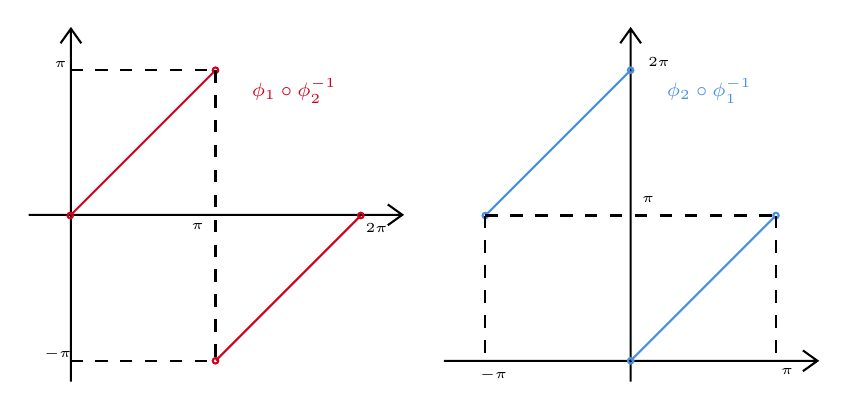
\begin{tikzpicture}[x=0.75pt,y=0.75pt,yscale=-1,xscale=1]
		%uncomment if require: \path (0,300); %set diagram left start at 0, and has height of 300
		
		%Shape: Axis 2D [id:dp031269396086308854] 
		\draw  (180,189.67) -- (360,189.67)(200.33,100) -- (200.33,270) (353,184.67) -- (360,189.67) -- (353,194.67) (195.33,107) -- (200.33,100) -- (205.33,107)  ;
		%Straight Lines [id:da8173483474090752] 
		\draw [color={rgb, 255:red, 208; green, 2; blue, 27 }  ,draw opacity=1 ][line width=0.75]    (200.24,189.76) -- (269.76,120.24) ;
		\draw [shift={(270,120)}, rotate = 315] [color={rgb, 255:red, 208; green, 2; blue, 27 }  ,draw opacity=1 ][line width=0.75]      (0, 0) circle [x radius= 1.34, y radius= 1.34]   ;
		\draw [shift={(200,190)}, rotate = 315] [color={rgb, 255:red, 208; green, 2; blue, 27 }  ,draw opacity=1 ][line width=0.75]      (0, 0) circle [x radius= 1.34, y radius= 1.34]   ;
		%Straight Lines [id:da7972743834901372] 
		\draw [color={rgb, 255:red, 208; green, 2; blue, 27 }  ,draw opacity=1 ][line width=0.75]    (270.24,259.76) -- (339.76,190.24) ;
		\draw [shift={(340,190)}, rotate = 315] [color={rgb, 255:red, 208; green, 2; blue, 27 }  ,draw opacity=1 ][line width=0.75]      (0, 0) circle [x radius= 1.34, y radius= 1.34]   ;
		\draw [shift={(270,260)}, rotate = 315] [color={rgb, 255:red, 208; green, 2; blue, 27 }  ,draw opacity=1 ][line width=0.75]      (0, 0) circle [x radius= 1.34, y radius= 1.34]   ;
		%Straight Lines [id:da11749218813373297] 
		\draw  [dash pattern={on 4.5pt off 4.5pt}]  (270,120) -- (270,260) ;
		%Shape: Axis 2D [id:dp7242837319994968] 
		\draw  (380,260) -- (560,260)(470,100) -- (470,270) (553,255) -- (560,260) -- (553,265) (465,107) -- (470,100) -- (475,107)  ;
		%Straight Lines [id:da7954245800299584] 
		\draw [color={rgb, 255:red, 74; green, 144; blue, 226 }  ,draw opacity=1 ][line width=0.75]    (400.24,189.76) -- (469.76,120.24) ;
		\draw [shift={(470,120)}, rotate = 315] [color={rgb, 255:red, 74; green, 144; blue, 226 }  ,draw opacity=1 ][line width=0.75]      (0, 0) circle [x radius= 1.34, y radius= 1.34]   ;
		\draw [shift={(400,190)}, rotate = 315] [color={rgb, 255:red, 74; green, 144; blue, 226 }  ,draw opacity=1 ][line width=0.75]      (0, 0) circle [x radius= 1.34, y radius= 1.34]   ;
		%Straight Lines [id:da15608839189923596] 
		\draw [color={rgb, 255:red, 74; green, 144; blue, 226 }  ,draw opacity=1 ][line width=0.75]    (470.24,259.76) -- (539.76,190.24) ;
		\draw [shift={(540,190)}, rotate = 315] [color={rgb, 255:red, 74; green, 144; blue, 226 }  ,draw opacity=1 ][line width=0.75]      (0, 0) circle [x radius= 1.34, y radius= 1.34]   ;
		\draw [shift={(470,260)}, rotate = 315] [color={rgb, 255:red, 74; green, 144; blue, 226 }  ,draw opacity=1 ][line width=0.75]      (0, 0) circle [x radius= 1.34, y radius= 1.34]   ;
		%Straight Lines [id:da8863860410352722] 
		\draw  [dash pattern={on 4.5pt off 4.5pt}]  (400,190) -- (400,260) ;
		%Straight Lines [id:da8092780134149673] 
		\draw  [dash pattern={on 4.5pt off 4.5pt}]  (540,190) -- (540,260) ;
		%Straight Lines [id:da9907647632614371] 
		\draw  [dash pattern={on 4.5pt off 4.5pt}]  (400,190) -- (540,190) ;
		%Straight Lines [id:da6719155425075689] 
		\draw  [dash pattern={on 4.5pt off 4.5pt}]  (200,260) -- (270,260) ;
		%Straight Lines [id:da26461137148185054] 
		\draw  [dash pattern={on 4.5pt off 4.5pt}]  (200,120) -- (270,120) ;
		
		% Text Node
		\draw (257,192.4) node [anchor=north west][inner sep=0.75pt]  [font=\tiny]  {$\pi $};
		% Text Node
		\draw (286,122.4) node [anchor=north west][inner sep=0.75pt]  [font=\scriptsize,color={rgb, 255:red, 208; green, 2; blue, 27 }  ,opacity=1 ]  {$\phi _{1} \circ \phi _{2}^{-1}$};
		% Text Node
		\draw (341,192.4) node [anchor=north west][inner sep=0.75pt]  [font=\tiny]  {$2\pi $};
		% Text Node
		\draw (396,262.4) node [anchor=north west][inner sep=0.75pt]  [font=\tiny]  {$-\pi $};
		% Text Node
		\draw (486,122.4) node [anchor=north west][inner sep=0.75pt]  [font=\scriptsize,color={rgb, 255:red, 74; green, 144; blue, 226 }  ,opacity=1 ]  {$\phi _{2} \circ \phi _{1}^{-1}$};
		% Text Node
		\draw (541,262.4) node [anchor=north west][inner sep=0.75pt]  [font=\tiny]  {$\pi $};
		% Text Node
		\draw (474,179.4) node [anchor=north west][inner sep=0.75pt]  [font=\tiny]  {$\pi $};
		% Text Node
		\draw (477,112.4) node [anchor=north west][inner sep=0.75pt]  [font=\tiny]  {$2\pi $};
		% Text Node
		\draw (191,114.4) node [anchor=north west][inner sep=0.75pt]  [font=\tiny]  {$\pi $};
		% Text Node
		\draw (186,252.4) node [anchor=north west][inner sep=0.75pt]  [font=\tiny]  {$-\pi $};
		
		
	\end{tikzpicture}
\end{figure}
	
\end{solution}

\begin{observation}
	I was thinking about my solution to the problem above, and I thought it is wrong, as I was thinking that the function $ \phi_1 $ is not homeomorphism as it is not continuous. But the point that I was missing is that this function is indeed continuous on its domain and the point of discontinuity (i.e. $ x = \pi $) is not in the domain. 
\end{observation}

\begin{problem}{Another $ C^\infty $ atlas on a circle}
	\label{problem:S^1Charts}
	In the previous problem, we constructed an atlas for a unit circle siting in the complex plane. In this problem we are going to construct a different atlas for a unit circle siting in the $ x-y $ plane. The following diagram are the charts for this unit circle. Write these charts explicitly and check if they are pairwise compatible.
	\begin{figure}[h!]
	
	
	\centering
	\tikzset{every picture/.style={line width=0.75pt}} %set default line width to 0.75pt        
	
	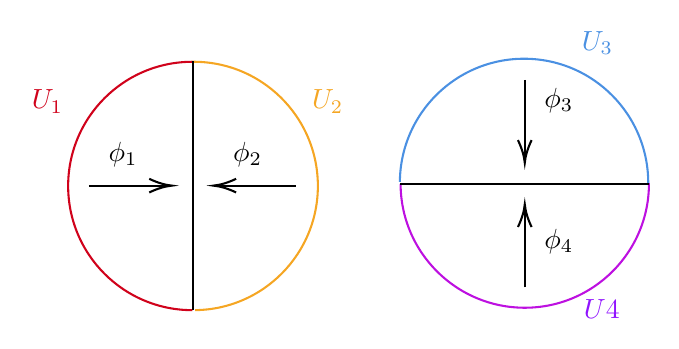
\begin{tikzpicture}[x=0.75pt,y=0.75pt,yscale=-1,xscale=1]
		%uncomment if require: \path (0,300); %set diagram left start at 0, and has height of 300
		
		%Shape: Arc [id:dp023481932229717062] 
		\draw  [draw opacity=0] (199.83,250) .. controls (199.83,250) and (199.83,250) .. (199.83,250) .. controls (199.83,250) and (199.83,250) .. (199.83,250) .. controls (166.79,250) and (140,223.21) .. (140,190.17) .. controls (140,157.12) and (166.79,130.33) .. (199.83,130.33) -- (199.83,190.17) -- cycle ; \draw  [color={rgb, 255:red, 208; green, 2; blue, 27 }  ,draw opacity=1 ] (199.83,250) .. controls (199.83,250) and (199.83,250) .. (199.83,250) .. controls (199.83,250) and (199.83,250) .. (199.83,250) .. controls (166.79,250) and (140,223.21) .. (140,190.17) .. controls (140,157.12) and (166.79,130.33) .. (199.83,130.33) ;  
		%Shape: Arc [id:dp8279857043077765] 
		\draw  [draw opacity=0] (199.83,130.33) .. controls (199.83,130.33) and (199.83,130.33) .. (199.83,130.33) .. controls (232.88,129.98) and (259.95,156.47) .. (260.31,189.52) .. controls (260.67,222.56) and (234.17,249.64) .. (201.13,249.99) -- (200.48,190.16) -- cycle ; \draw  [color={rgb, 255:red, 245; green, 166; blue, 35 }  ,draw opacity=1 ] (199.83,130.33) .. controls (199.83,130.33) and (199.83,130.33) .. (199.83,130.33) .. controls (232.88,129.98) and (259.95,156.47) .. (260.31,189.52) .. controls (260.67,222.56) and (234.17,249.64) .. (201.13,249.99) ;  
		%Shape: Arc [id:dp2277450931666709] 
		\draw  [draw opacity=0] (299.82,188.21) .. controls (299.82,188.21) and (299.82,188.21) .. (299.82,188.21) .. controls (300.08,155.16) and (327.08,128.59) .. (360.13,128.86) .. controls (393.17,129.12) and (419.75,156.12) .. (419.48,189.17) -- (359.65,188.69) -- cycle ; \draw  [color={rgb, 255:red, 74; green, 144; blue, 226 }  ,draw opacity=1 ] (299.82,188.21) .. controls (299.82,188.21) and (299.82,188.21) .. (299.82,188.21) .. controls (300.08,155.16) and (327.08,128.59) .. (360.13,128.86) .. controls (393.17,129.12) and (419.75,156.12) .. (419.48,189.17) ;  
		%Shape: Arc [id:dp16056893747855794] 
		\draw  [draw opacity=0] (419.83,188.83) .. controls (419.83,188.83) and (419.83,188.83) .. (419.83,188.83) .. controls (419.93,221.88) and (393.21,248.74) .. (360.17,248.83) .. controls (327.12,248.93) and (300.26,222.21) .. (300.17,189.17) -- (360,189) -- cycle ; \draw  [color={rgb, 255:red, 189; green, 16; blue, 224 }  ,draw opacity=1 ] (419.83,188.83) .. controls (419.83,188.83) and (419.83,188.83) .. (419.83,188.83) .. controls (419.93,221.88) and (393.21,248.74) .. (360.17,248.83) .. controls (327.12,248.93) and (300.26,222.21) .. (300.17,189.17) ;  
		%Straight Lines [id:da9947609889928073] 
		\draw    (150,190) -- (188,190) ;
		\draw [shift={(190,190)}, rotate = 180] [color={rgb, 255:red, 0; green, 0; blue, 0 }  ][line width=0.75]    (10.93,-3.29) .. controls (6.95,-1.4) and (3.31,-0.3) .. (0,0) .. controls (3.31,0.3) and (6.95,1.4) .. (10.93,3.29)   ;
		%Straight Lines [id:da6553860547904606] 
		\draw    (212,190) -- (250,190) ;
		\draw [shift={(210,190)}, rotate = 0] [color={rgb, 255:red, 0; green, 0; blue, 0 }  ][line width=0.75]    (10.93,-3.29) .. controls (6.95,-1.4) and (3.31,-0.3) .. (0,0) .. controls (3.31,0.3) and (6.95,1.4) .. (10.93,3.29)   ;
		%Straight Lines [id:da19474028508083085] 
		\draw    (360,139) -- (360,177) ;
		\draw [shift={(360,179)}, rotate = 270] [color={rgb, 255:red, 0; green, 0; blue, 0 }  ][line width=0.75]    (10.93,-3.29) .. controls (6.95,-1.4) and (3.31,-0.3) .. (0,0) .. controls (3.31,0.3) and (6.95,1.4) .. (10.93,3.29)   ;
		%Straight Lines [id:da648683487634115] 
		\draw    (360,239) -- (360,201) ;
		\draw [shift={(360,199)}, rotate = 90] [color={rgb, 255:red, 0; green, 0; blue, 0 }  ][line width=0.75]    (10.93,-3.29) .. controls (6.95,-1.4) and (3.31,-0.3) .. (0,0) .. controls (3.31,0.3) and (6.95,1.4) .. (10.93,3.29)   ;
		%Straight Lines [id:da9130830416071034] 
		\draw    (200,130) -- (200,250) ;
		%Straight Lines [id:da1322223309435544] 
		\draw    (420,189) -- (300,189) ;
		
		% Text Node
		\draw (121,142.4) node [anchor=north west][inner sep=0.75pt]  [color={rgb, 255:red, 208; green, 2; blue, 27 }  ,opacity=1 ]  {$U_{1}$};
		% Text Node
		\draw (256,142.4) node [anchor=north west][inner sep=0.75pt]  [color={rgb, 255:red, 245; green, 166; blue, 35 }  ,opacity=1 ]  {$U_{2}$};
		% Text Node
		\draw (386,114.4) node [anchor=north west][inner sep=0.75pt]  [color={rgb, 255:red, 74; green, 144; blue, 226 }  ,opacity=1 ]  {$U_{3}$};
		% Text Node
		\draw (387,243.4) node [anchor=north west][inner sep=0.75pt]  [color={rgb, 255:red, 144; green, 19; blue, 254 }  ,opacity=1 ]  {$U4$};
		% Text Node
		\draw (158,167.4) node [anchor=north west][inner sep=0.75pt]    {$\phi _{1}$};
		% Text Node
		\draw (218,167.4) node [anchor=north west][inner sep=0.75pt]    {$\phi _{2}$};
		% Text Node
		\draw (368,141.4) node [anchor=north west][inner sep=0.75pt]    {$\phi _{3}$};
		% Text Node
		\draw (368,209.4) node [anchor=north west][inner sep=0.75pt]    {$\phi _{4}$};
		
		
	\end{tikzpicture}
\end{figure}

\FloatBarrier
\end{problem}
\begin{solution}
	The explicit formulas for the charts depicted above is as following
	\[ (U_1, \phi_1:U_1\to \R),(U_2, \phi_2:U_2\to \R), (U_3, \phi_3:U_3\to \R),(U_4, \phi_4:U_4\to \R), \]
	where we have
	\[ \phi_1(x,y) = y,\qquad  \phi_2(x,y) = y, \qquad \phi_3(x,y) = x, \qquad \phi_4(x,y) = x. \]
	Note that although some of the functions above might have a same formula, but they are different functions as they have different domains. To show that these functions are pairwise compatible, we start by noting that since $ U_1 \cap U_2 = \emptyset $, thus $ (U_1,\phi_1) $ and $ (U_2,\phi_2) $ are compatible. With the same reasoning, the charts $ (U_3,\phi_3) $ and $ (U_4,\phi_4) $ are compatible. Now, we want to show that $ (U_1,\phi_1) $ is compatible with $ (U_3,\phi_3) $. We need to show that 
	\[ \phi_1 \circ \inv{\phi_3}: \underbrace{\phi_3(U_1\cap U_3)}_{(-1,0)} \to \underbrace{\phi_1(U_1\cap U_3)}_{(0,1)}\quad \text{and} \quad \phi_3\circ \inv{\phi_1}:\underbrace{\phi_1(U_1\cap U_3)}_{(0,1)} \to \underbrace{\phi_3(U_1\cap  U_3)}_{(-1,0)} \]
	are $ C^\infty $. To write them explicitly, we have
	\[ (\phi_1 \circ \inv{\phi_3})(x) = \phi_1(x,\sqrt{1-x^2}) = \sqrt{1-x^2}.  \]
	Also
	\[ (\phi_3 \circ \inv{\phi_1})(x) = \phi_3(-\sqrt{1-x^2},x) = -\sqrt{1-x^2}. \]
	We can see that both of these functions are $ C^\infty $ in their domain. Now, for the charts $ (U_1, \phi_1) $ and $ (U_4,\phi_4) $ need to show
	\[ \phi_1 \circ \inv{\phi_4}:\underbrace{ \phi_4(U_1\cap U_4)}_{(-1,0)} \to \underbrace{\phi_1(U_1\cap U_4)}_{(-1,0)} \qquad \text{and} \qquad \phi_4\circ \inv{\phi_1}: \underbrace{\phi_1(U_1\cap U_4)}_{(-1,0)} \to  \underbrace{\phi_4(U_1\cap U_4)}_{(-1,0)} \]
	are $ C^\infty $ in their domain. Explicitly, we have
	\[ (\phi_1 \circ \inv{\phi_4})(x) = -\sqrt{1 -x^2}, \qquad (\phi_4\circ \inv{\phi_1})(x) = -\sqrt{1-x^2}.\]
	With the same strategy, we can show that this collection of charts indeed makes a $ C^\infty $ atlas for the unit circle in $ x-y $ plane.
\end{solution}


\begin{problem}[The real line with two origins (from W. Tu)]
	Let $ A $ and $ B $ be two points not on the real line $ \R $. Consider the set $ S = (\R - \set{0}) \cup \set{A,B} $. For nay two positive real numbers $ c,d $, define 
	\[ I_A(-c,d) = (-c,0) \cup \set{A} \cap (0,d) \]
	and similarly for $ I_B(-c,d) $, with $ B $ instead of $ A $. Define a topology on $ S $ as follows: On $ (\R - \set{0}) $, use the subspace topology inherited from $ \R $, with open intervals as a basis. A basis of neighborhoods at $ A $ is the set $ \set{I_A(-c,d)\ |\ c,d > 0} $; similarly, a basis of neighborhoods at $ B $ is $ \set{I_B(-c,d)\ |\ c,d > 0} $.
	\begin{enumerate}[(a)]
		\item Prove that the map $ h: I_A(-c,d) \to (-c,d) $ defined by
		\begin{align*}
			h(x)&=x \qquad \text{for}\ x\in(-c,0) \cup (0,d),\\
			h(A)&=0
		\end{align*}
		is a homeomorphism.
		
		\item Show that $ S $ is locally Euclidean and second countable, but not Hausdorff.
	\end{enumerate}
\end{problem}

\begin{solution}
	\begin{enumerate}[(a)]
		\item We need to show that $ h $ is one-to-one, onto, and continuous, with continuous inverse. To show being one-to-one, let $ x,y \in I_A(-c,d) $ such that $ x\neq y $ and possibly one of them equal to $ A $. If none is equal to $ A $, then $ h $ is the identity map which is one-to-one. However, if one of them is equal to $ A $, let's say $ x = A $, then $ h(x) = 0 $ where $ h(y) \in (-c,d)\cup(0,d)$, thus $ h(y) \neq 0 $. This proves that $ h $ is indeed one to one. To show that the function is onto, let $ z \in (-c,d) $. Then if $ z = 0 $ we have $ h(A) = z $, and if $ z \neq 0 $, we have $ h(z) = z $. Thus the function $ h $ is a bijection.
		
		As the second step, we need to show that this function is continuous with continuous inverse. From definition of continuoity, we just need to show that both $ h $ and $ \inv{h} $ maps opens to opens (because for continuous function the pre-image of every open set is an open set; and to show that the inverse of the function is also continuous we need to show that the image of every open is also open).
		Let $ U = (a,b) \subset I_A(-c,d) $ be an open set in the topology of $ S $. If $ A \notin (a,b) $, then the image of this set under $ h $ is $ (a,b) $ which is open in $ (-c,d) $. But if $ A \in (a,b) $, then the image of this set under the map $ h $ is $ (a,0)\cup(0,b)\cup\set{0} = (a,b) $, which is also open. Thus $ \inv{h} $ is continuous. To show the continuity of $ \inv{h} $, let $ (a,b) \subset (c,d) $. If $ 0 \notin (a,b) $, then pre-image of this set under the map $ f $ is $ (a,b) $ that is open in $ S $. However if $ 0 \in (a,b) $, then the pre-image of this set under $ f $ is the set $ (-a,0) \cup \set{A} \cup (0,b) $ which is indeed open in $ S $ as we can construct this with the basis if opens at $ A $.
		
		\item First, we show that $ S $ is locally Euclidean. To show this let $ p \in S $. If $ p \neq A $ and $ p \neq B $, then we choose an open set $ U =  (a,b) $ containing $ p $ that does not contain neither of $ A $ and  $ B $. Then $ U $ is homeomorphic to $ (a,b) $ with the identity map. However if $ p = A $, we choose any open $ U = (a,b) $ containing $ p $. Then $ (U = (a,b),I_A(a,b)) $ is a local chart. For the case where $ p = B $, we can find a suitable chart with the same reasoning as for $ A $. Thus we have shown that $ S $ is locally Euclidean.
		
		To show that $ S $ is second countable, let $ \mathcal{B} $ be a basis for $ \R - \set{0} $. Since $ \R $ is second countable, then $ \mathcal{B} $ is countable. Let $ \mathbb{B} = \mathcal{B} \cup I_A(-c,d) \cup I_B(-c,d) $ is a countable basis for $ S $ for some $ c,d > 0 $. This shows that $ S $ is also second countable.
		
		However, this space is not Hausdorff. To show this consider the points $ A,B $. We can not find any two open $ U,V $ such that $ A \in U $ and $ B \in V $ and we have $ U \cap V = \emptyset $. Or equivalently, for all open sets $ U,V $  such that $ A \in U $ and $ B \in V $ we have $ U\cap V \neq \emptyset $. That is because from the basis of the open neighborhoods at $ A,B $ we have $ U = I_A(-c,d) $ and $ V = I_B(-e,f) $ for some $ c,d,e,f > 0 $. It is clear that $ U \cap V \neq 0 $, thus $ S $ is not Hausdorff.
	\end{enumerate}
\end{solution}

\begin{problem}[A sphere with a hair (from W. Tu) ] 
	A fundamental theorem of topology, the theorem on invariance of dimension, states that if two nonempty open sets $ U \subset \R^n $ and $ V \subset \R^m $ are homeomorphic, then $ n = m $. Prove that the sphere with a hair in $ \R^3 $ is not locally Euclidean at $ q $ (the point that the hair attaches to the sphere). Hence it cannot be a topological manifold. 
\end{problem}

\begin{solution}
	We will proceed with the proof by contradiction. Assume that the ball with hair at  point $ q $ is homeomorphic to some open set in $ \R^n $. Then $ q $ has an open neighborhood $ U $ homeomorphic to an open ball $ B := \mathbb{B}(0,\epsilon) \in \R^n $, with $ q $ mapping to 0. We can restrict this homeomorphism to a homeomorphism $ U - \set{q} \to B - \set{0} $. Now $ B-\set{0} $ is either connected if $ n \geq 2 $ or has two connected components if $ n=1 $, where $ U - \set{q} $ has two connected components where one component is a 1 dimensional manifold (the hair) and the other component is a 2 dimensional manifold (the sphere). The only case where $ B - \set{0} $ has two connected components is when $ n = 1 $. But because of the invariance of dimension principle, the sphere (2 dimensional manifold) can not be homeomorphic to a one dimensional manifold. Thus there is no such a homeomorphism between the hairy ball and $ \R^n $ and the hairy ball is not locally Euclidean in $ q $.
\end{solution}

\begin{problem}[Charts on a sphere (from W. Tu)]
	Let $ S^2 $ be the unit sphere, i.e.
	\[ S^2 = \set{(x,y,z)\in\R^3\ :\ x^2+y^2+z^2 = 1} \]
	in $ \R^3 $. Define in $ S^2 $ the six charts corresponding to the six hemispheres (from the front, rear, right, left, upper, and lower hemispheres) as in the figure.
	\begin{align*}
		U_1 = \set{(x,y,z) \in S^2\ |\ x > 0}, \qquad \phi_1(x,y,z) = (y,z), \\
		U_2 = \set{(x,y,z) \in S^2\ |\ x < 0}, \qquad \phi_2(x,y,z) = (y,z), \\
		U_3 = \set{(x,y,z) \in S^2\ |\ y > 0}, \qquad \phi_3(x,y,z) = (x,z), \\
		U_4 = \set{(x,y,z) \in S^2\ |\ y < 0}, \qquad \phi_4(x,y,z) = (x,z), \\
		U_5 = \set{(x,y,z) \in S^2\ |\ z > 0}, \qquad \phi_5(x,y,z) = (x,y), \\
		U_6 = \set{(x,y,z) \in S^2\ |\ z < 0}, \qquad \phi_6(x,y,z) = (x,y).
	\end{align*}
	Note that although some of the functions above might look similar (like $ \phi_3 $ and $ \phi_4 $) but they are in fact different functions as they have different domains. Show that $ \phi_1\circ \inv{\phi_4}, \phi_4 \circ \inv{\phi_1} $ is $ C^\infty $ on $ \phi_4(U_1 \cap U_4), \phi_1(U_1 \cap U_4) $ respectively. Do the same same analysis for $ \phi_6 \circ \inv{\phi_1}$.
	\begin{figure}[h!]
	
	\centering
	
	\tikzset{every picture/.style={line width=0.75pt}} %set default line width to 0.75pt        
	
	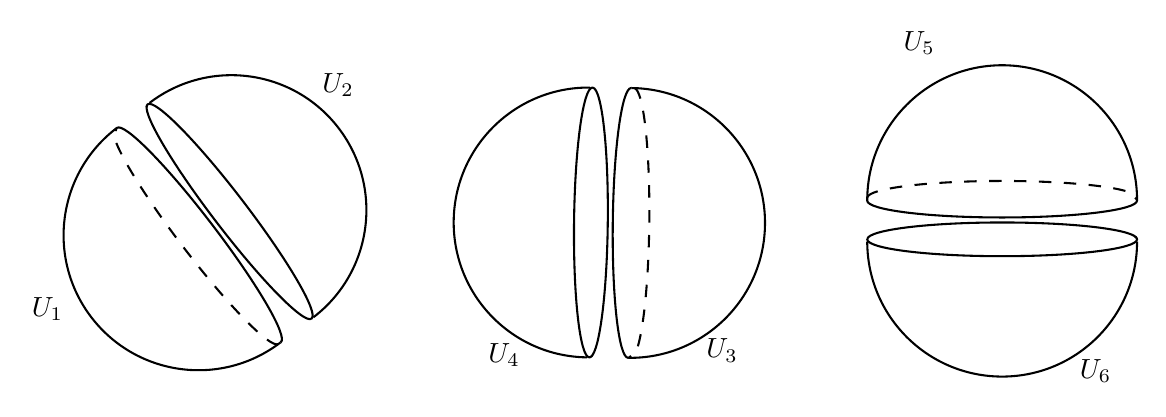
\begin{tikzpicture}[x=0.75pt,y=0.75pt,yscale=-1,xscale=1]
		%uncomment if require: \path (0,300); %set diagram left start at 0, and has height of 300
		
		%Shape: Arc [id:dp8087392079745468] 
		\draw  [draw opacity=0] (610,205) .. controls (610,205) and (610,205) .. (610,205) .. controls (610,240.9) and (580.9,270) .. (545,270) .. controls (509.1,270) and (480,240.9) .. (480,205) -- (545,205) -- cycle ; \draw   (610,205) .. controls (610,205) and (610,205) .. (610,205) .. controls (610,240.9) and (580.9,270) .. (545,270) .. controls (509.1,270) and (480,240.9) .. (480,205) ;  
		%Shape: Arc [id:dp7144643582066421] 
		\draw  [draw opacity=0] (480.02,203.67) .. controls (480.89,199.28) and (509.65,195.75) .. (545,195.75) .. controls (578.58,195.75) and (606.22,198.93) .. (609.64,203.02) -- (545,203.88) -- cycle ; \draw   (480.02,203.67) .. controls (480.89,199.28) and (509.65,195.75) .. (545,195.75) .. controls (578.58,195.75) and (606.22,198.93) .. (609.64,203.02) ;  
		%Shape: Arc [id:dp9774877190814104] 
		\draw  [draw opacity=0] (480,185) .. controls (480,185) and (480,185) .. (480,185) .. controls (480,149.1) and (509.1,120) .. (545,120) .. controls (580.9,120) and (610,149.1) .. (610,185) -- (545,185) -- cycle ; \draw   (480,185) .. controls (480,185) and (480,185) .. (480,185) .. controls (480,149.1) and (509.1,120) .. (545,120) .. controls (580.9,120) and (610,149.1) .. (610,185) ;  
		%Shape: Arc [id:dp7118645098131682] 
		\draw  [draw opacity=0] (609.09,202.51) .. controls (609.69,202.95) and (610,203.41) .. (610,203.88) .. controls (610,208.36) and (580.9,212) .. (545,212) .. controls (509.1,212) and (480,208.36) .. (480,203.88) .. controls (480,203.8) and (480.01,203.73) .. (480.02,203.66) -- (545,203.88) -- cycle ; \draw   (609.09,202.51) .. controls (609.69,202.95) and (610,203.41) .. (610,203.88) .. controls (610,208.36) and (580.9,212) .. (545,212) .. controls (509.1,212) and (480,208.36) .. (480,203.88) .. controls (480,203.8) and (480.01,203.73) .. (480.02,203.66) ;  
		%Shape: Arc [id:dp7962209595423704] 
		\draw  [draw opacity=0] (609.06,183.85) .. controls (609.66,184.29) and (609.98,184.75) .. (609.98,185.22) .. controls (609.98,189.7) and (580.88,193.34) .. (544.98,193.34) .. controls (509.08,193.34) and (479.98,189.7) .. (479.98,185.22) .. controls (479.98,185.14) and (479.99,185.07) .. (480,185) -- (544.98,185.22) -- cycle ; \draw   (609.06,183.85) .. controls (609.66,184.29) and (609.98,184.75) .. (609.98,185.22) .. controls (609.98,189.7) and (580.88,193.34) .. (544.98,193.34) .. controls (509.08,193.34) and (479.98,189.7) .. (479.98,185.22) .. controls (479.98,185.14) and (479.99,185.07) .. (480,185) ;  
		%Shape: Arc [id:dp26854896682720364] 
		\draw  [draw opacity=0][dash pattern={on 4.5pt off 4.5pt}] (480.02,183.67) .. controls (480.89,179.28) and (509.65,175.75) .. (545,175.75) .. controls (578.58,175.75) and (606.22,178.93) .. (609.64,183.02) -- (545,183.88) -- cycle ; \draw  [dash pattern={on 4.5pt off 4.5pt}] (480.02,183.67) .. controls (480.89,179.28) and (509.65,175.75) .. (545,175.75) .. controls (578.58,175.75) and (606.22,178.93) .. (609.64,183.02) ;  
		%Shape: Arc [id:dp8593027572319052] 
		\draw  [draw opacity=0] (345,260.74) .. controls (345,260.74) and (345,260.74) .. (345,260.74) .. controls (345,260.74) and (345,260.74) .. (345,260.74) .. controls (309.1,260.33) and (280.34,230.89) .. (280.75,195) .. controls (281.16,159.1) and (310.6,130.34) .. (346.49,130.75) -- (345.74,195.74) -- cycle ; \draw   (345,260.74) .. controls (345,260.74) and (345,260.74) .. (345,260.74) .. controls (345,260.74) and (345,260.74) .. (345,260.74) .. controls (309.1,260.33) and (280.34,230.89) .. (280.75,195) .. controls (281.16,159.1) and (310.6,130.34) .. (346.49,130.75) ;  
		%Shape: Arc [id:dp5017110012711772] 
		\draw  [draw opacity=0] (347.82,130.78) .. controls (352.2,131.7) and (355.4,160.5) .. (354.99,195.85) .. controls (354.61,229.43) and (351.11,257.03) .. (346.98,260.41) -- (346.87,195.76) -- cycle ; \draw   (347.82,130.78) .. controls (352.2,131.7) and (355.4,160.5) .. (354.99,195.85) .. controls (354.61,229.43) and (351.11,257.03) .. (346.98,260.41) ;  
		%Shape: Arc [id:dp34022749055732393] 
		\draw  [draw opacity=0] (366.49,130.98) .. controls (366.49,130.98) and (366.49,130.98) .. (366.49,130.98) .. controls (402.39,131.39) and (431.15,160.83) .. (430.74,196.72) .. controls (430.33,232.62) and (400.89,261.38) .. (364.99,260.97) -- (365.74,195.97) -- cycle ; \draw   (366.49,130.98) .. controls (366.49,130.98) and (366.49,130.98) .. (366.49,130.98) .. controls (402.39,131.39) and (431.15,160.83) .. (430.74,196.72) .. controls (430.33,232.62) and (400.89,261.38) .. (364.99,260.97) ;  
		%Shape: Arc [id:dp9156415467589833] 
		\draw  [draw opacity=0] (347.5,259.86) .. controls (347.05,260.45) and (346.59,260.76) .. (346.12,260.75) .. controls (341.63,260.7) and (338.33,231.56) .. (338.74,195.66) .. controls (339.16,159.77) and (343.13,130.71) .. (347.62,130.76) .. controls (347.69,130.76) and (347.76,130.77) .. (347.83,130.79) -- (346.87,195.76) -- cycle ; \draw   (347.5,259.86) .. controls (347.05,260.45) and (346.59,260.76) .. (346.12,260.75) .. controls (341.63,260.7) and (338.33,231.56) .. (338.74,195.66) .. controls (339.16,159.77) and (343.13,130.71) .. (347.62,130.76) .. controls (347.69,130.76) and (347.76,130.77) .. (347.83,130.79) ;  
		%Shape: Arc [id:dp7534866185784517] 
		\draw  [draw opacity=0] (366.15,260.05) .. controls (365.7,260.64) and (365.24,260.95) .. (364.78,260.95) .. controls (360.29,260.89) and (356.99,231.75) .. (357.4,195.86) .. controls (357.82,159.96) and (361.79,130.9) .. (366.28,130.95) .. controls (366.35,130.96) and (366.42,130.96) .. (366.49,130.98) -- (365.53,195.95) -- cycle ; \draw   (366.15,260.05) .. controls (365.7,260.64) and (365.24,260.95) .. (364.78,260.95) .. controls (360.29,260.89) and (356.99,231.75) .. (357.4,195.86) .. controls (357.82,159.96) and (361.79,130.9) .. (366.28,130.95) .. controls (366.35,130.96) and (366.42,130.96) .. (366.49,130.98) ;  
		%Shape: Arc [id:dp7058755896129407] 
		\draw  [draw opacity=0][dash pattern={on 4.5pt off 4.5pt}] (367.82,131.01) .. controls (372.2,131.93) and (375.4,160.73) .. (374.99,196.08) .. controls (374.61,229.66) and (371.1,257.26) .. (366.98,260.64) -- (366.87,195.99) -- cycle ; \draw  [dash pattern={on 4.5pt off 4.5pt}] (367.82,131.01) .. controls (372.2,131.93) and (375.4,160.73) .. (374.99,196.08) .. controls (374.61,229.66) and (371.1,257.26) .. (366.98,260.64) ;  
		%Shape: Arc [id:dp6580687340920708] 
		\draw  [draw opacity=0] (134.21,138.15) .. controls (134.21,138.15) and (134.21,138.15) .. (134.21,138.15) .. controls (134.21,138.15) and (134.21,138.15) .. (134.21,138.15) .. controls (162.73,116.35) and (203.52,121.79) .. (225.32,150.31) .. controls (247.13,178.82) and (241.69,219.62) .. (213.17,241.42) -- (173.69,189.79) -- cycle ; \draw   (134.21,138.15) .. controls (134.21,138.15) and (134.21,138.15) .. (134.21,138.15) .. controls (134.21,138.15) and (134.21,138.15) .. (134.21,138.15) .. controls (162.73,116.35) and (203.52,121.79) .. (225.32,150.31) .. controls (247.13,178.82) and (241.69,219.62) .. (213.17,241.42) ;  
		%Shape: Arc [id:dp04807301977746614] 
		\draw  [draw opacity=0] (212.1,242.21) .. controls (208.08,244.19) and (187.81,223.49) .. (166.34,195.4) .. controls (145.94,168.73) and (131.69,144.84) .. (132.85,139.64) -- (172.79,190.47) -- cycle ; \draw   (212.1,242.21) .. controls (208.08,244.19) and (187.81,223.49) .. (166.34,195.4) .. controls (145.94,168.73) and (131.69,144.84) .. (132.85,139.64) ;  
		%Shape: Arc [id:dp5373023961242778] 
		\draw  [draw opacity=0] (197.28,253.57) .. controls (197.28,253.57) and (197.28,253.57) .. (197.28,253.57) .. controls (197.28,253.57) and (197.28,253.57) .. (197.28,253.57) .. controls (168.76,275.37) and (127.97,269.93) .. (106.16,241.41) .. controls (84.36,212.89) and (89.8,172.1) .. (118.32,150.3) -- (157.8,201.93) -- cycle ; \draw   (197.28,253.57) .. controls (197.28,253.57) and (197.28,253.57) .. (197.28,253.57) .. controls (197.28,253.57) and (197.28,253.57) .. (197.28,253.57) .. controls (168.76,275.37) and (127.97,269.93) .. (106.16,241.41) .. controls (84.36,212.89) and (89.8,172.1) .. (118.32,150.3) ;  
		%Shape: Arc [id:dp6075301311311689] 
		\draw  [draw opacity=0] (132.79,140.39) .. controls (132.77,139.64) and (132.95,139.11) .. (133.31,138.83) .. controls (136.88,136.11) and (157.44,157.02) .. (179.25,185.53) .. controls (201.05,214.05) and (215.84,239.38) .. (212.27,242.11) .. controls (212.22,242.15) and (212.15,242.19) .. (212.09,242.22) -- (172.79,190.47) -- cycle ; \draw   (132.79,140.39) .. controls (132.77,139.64) and (132.95,139.11) .. (133.31,138.83) .. controls (136.88,136.11) and (157.44,157.02) .. (179.25,185.53) .. controls (201.05,214.05) and (215.84,239.38) .. (212.27,242.11) .. controls (212.22,242.15) and (212.15,242.19) .. (212.09,242.22) ;  
		%Shape: Arc [id:dp4893987696896971] 
		\draw  [draw opacity=0] (117.98,151.74) .. controls (117.96,150.99) and (118.14,150.47) .. (118.5,150.18) .. controls (122.07,147.46) and (142.64,168.37) .. (164.44,196.89) .. controls (186.24,225.4) and (201.03,250.73) .. (197.46,253.46) .. controls (197.41,253.5) and (197.34,253.54) .. (197.28,253.57) -- (157.98,201.82) -- cycle ; \draw   (117.98,151.74) .. controls (117.96,150.99) and (118.14,150.47) .. (118.5,150.18) .. controls (122.07,147.46) and (142.64,168.37) .. (164.44,196.89) .. controls (186.24,225.4) and (201.03,250.73) .. (197.46,253.46) .. controls (197.41,253.5) and (197.34,253.54) .. (197.28,253.57) ;  
		%Shape: Arc [id:dp5010740042347757] 
		\draw  [draw opacity=0][dash pattern={on 4.5pt off 4.5pt}] (196.21,254.36) .. controls (192.19,256.34) and (171.92,235.64) .. (150.45,207.55) .. controls (130.05,180.87) and (115.8,156.99) .. (116.96,151.78) -- (156.91,202.62) -- cycle ; \draw  [dash pattern={on 4.5pt off 4.5pt}] (196.21,254.36) .. controls (192.19,256.34) and (171.92,235.64) .. (150.45,207.55) .. controls (130.05,180.87) and (115.8,156.99) .. (116.96,151.78) ;  
		
		% Text Node
		\draw (76,230.4) node [anchor=north west][inner sep=0.75pt]    {$U_{1}$};
		% Text Node
		\draw (216,122.4) node [anchor=north west][inner sep=0.75pt]    {$U_{2}$};
		% Text Node
		\draw (401,250.4) node [anchor=north west][inner sep=0.75pt]    {$U_{3}$};
		% Text Node
		\draw (296,252.4) node [anchor=north west][inner sep=0.75pt]    {$U_{4}$};
		% Text Node
		\draw (496,102.4) node [anchor=north west][inner sep=0.75pt]    {$U_{5}$};
		% Text Node
		\draw (581,260.4) node [anchor=north west][inner sep=0.75pt]    {$U_{6}$};
		
		
	\end{tikzpicture}
\end{figure}
\end{problem}
\begin{solution}
	For the set $ U_1 \cap U_4 $ we have
	\[ U_1 \cap U_4 = \set{(x,y,z) \in S^2\ :\ x>0 \text{ and } y < 0 }. \]
	Thus we will have
	\[ \phi_4(U_1\cap U_4) = \set{(x,z)\in \R^2 \ :\ x^2 + z^2 \leq 1,\ x>0}. \]
	Thus we can write
	\[ (\phi_1 \circ \inv{\phi_4})(\langle x,z \rangle ) = \phi_1(\langle x,-\sqrt{1-(x^2+y^2)},z \rangle) = \langle -\sqrt{1-(x^2+y^2)},z \rangle  \]
	This is indeed a $ C^\infty $ vector valued function, since each component is a $ C^\infty $ function. Now to evaluate $ \phi_4 \circ \inv{\phi_1}: \phi_1(U_1 \cap U_4) \to \phi_4(U_1\cap U_4) $ we need to first evaluate the set $ \phi_1(U_1 \cap U_4) $. For this set we have
	\[ \phi_1(U_1 \cap U_4) = \set{(z,y)\in\R^2\ :\ z^2 + y^2 \leq 1, y < 0}. \]
	Then we can write
	\[ (\phi_4 \circ \inv{\phi_1})(\langle y,z \rangle ) = \phi_4(\langle \sqrt{1-(y^2+z^2)}, y,z  \rangle) = \langle \sqrt{1-(y^2+z^2)} , z \rangle. \]
	This is indeed a $ C^\infty $ vector valued function. 
	
	To evaluate the function $ \phi_6 \circ \inv{\phi}_1: \phi_1(U_1 \cap U_6) \to \phi_6(U_1 \cap U_6) $, we first need to determine the domain of this function. First observe that 
	\[ U_1 \cap U_6 =  \set{(x,y,z) \in S^2\ :\ x>0 \text{ and } y<0}, \]
	which is the same as $ U_1 \cap U_4 $. Then for the domain of the function of interest we can write
	\[ \phi_1(U_1 \cap U_6) = \set{(y,z) \in \R^2 :\ z^2 + y^2 \leq 1 \text{ and } y<0}, \]
	\[ (\phi_6 \circ \inv{\phi_1})(\langle y,z \rangle) = \phi_6(\langle \sqrt{1-(y^2+z^2)},y,z \rangle) = \langle \sqrt{1-(y^2+z^2)}, y \rangle. \]
\end{solution}

\begin{problem}[Existence of a coordinate neighborhood (from W. Tu)]
	Let $ \set{(U_\alpha, \phi_\alpha)}_{\alpha \in I} $ be the maximal atlas on manifold $ M $. For any open set $ U $ in $ M $ and a point $ p \in U $, prove the existence of a coordinate open set $ U_\alpha $ such that $ p \in U_\alpha \subset U $.
\end{problem}
\begin{solution}
	Since $ \set{(U_\alpha,\phi_\alpha)}_{\alpha \in I} $ is an atlas, then for $ p \in U $ given as above, we can find some $ \alpha_1 \in I $ such that $ p \in U_{\alpha_1} $. Consider the open set $ W = U_{\alpha_1} \cap U $. The chart $ (W, \phi_{\alpha_1}|_W) $ is in the atlas (since it is maximal), i.e. $ \exists \alpha \in I $ such that $ (U_\alpha, \phi_\alpha) = (W, \phi_{\alpha_1}|_W) $. This completes the proof.
\end{solution}

\begin{problem}[An atlas for a product manifold (from W. Tu)]
	Prove the following proposition.
	\begin{proposition}
		If $ \set{(U_\alpha,\phi_\alpha)} $ and $ \set{(V_i,\psi_i)} $ are $ C^\infty $ atlases for the manifold $ M $ and $ N $ of dimensions $ m $ and $ n $, respectively, then the collection 
		\[ \set{(U_\alpha \times V_i,\phi_\alpha \times \psi_i)} \] where
		\[ \phi_\alpha \times \psi_i\ :\ U_\alpha \times V_i \to \R^m \times \R^n \]
		of charts is a $ C^\infty $ atlas on $ M\times N $. Therefore, $ M\times N $ is a $ C^\infty $ manifold of dimension $ m+n $.
	\end{proposition}
\end{problem}
\begin{solution}
	In order to show that the collection $ \frak{U} = \set{(U_\alpha \times V_i, \phi_\alpha \times \psi_i)} $ is an atlas for $ M\times N $, we need to show that charts are pairwise compatible as well as the set covering the whole space. To show that the chart covers the whole space $ M\times N $, let $ (p_1,p_2) \in M\times N $. Then $ p_1 \in M $ and $ p_2 \in N $. Then there are two coordinate open sets such that $ p_1 \in U_{\alpha_1} $ and $ p_2 \in V_{i_1} $. Thus the coordinate open set $ U_{\alpha_1} \times V_{i_1} $ contains the point $ (p_1,p_2) $.
	
	To show that two any two charts in the collection $ \frak{U} $ are compatible, let $ (U_{\alpha_1} \times V_{i_1},\phi_{\alpha_1}\times \psi_{i_1}) $ and $  (U_{\alpha_2} \times V_{i_2},\phi_{\alpha_2}\times \psi_{i_2}) $ be two  charts. We claim that the corresponding coordinate maps are $ C^\infty $. This follows directly from the fact the each component of the map these coordinate maps are $ C^\infty $.
\end{solution}

\begin{problem}[Smoothness of a projection map (from W. Tu)]
	Let $ M $ and $ N $ be manifolds and $ \pi: M\times N \to M $, $ \pi(p,q) = p $ the projection to the first factor. Prove that $ \pi $ is a $ C^\infty $ map.
\end{problem}

\begin{solution}
	Let $ p \in M $ and $ q \in N $, thus $ (p,q) \in M\times N $. Let $ \phi $ and $ \psi $ be two coordinate maps such that $ \phi(p) = x $ and $ \psi(q) = y $. Thus we can write $ (\phi, \psi)(p,q) = (x,y) $. Consider the function
	\[ (\phi \circ \pi \circ (\phi\times \psi)^{-1})(x,y) = \phi(\pi(p,q)) = \phi(p) = x.  \]
	The function above is a $ \C^\infty $ map from $ \R^{n+m} $ to $ \R^n $ (assuming $ M, N $ are $ m $ and $ n $ dimensional manifolds). This proves that the projection map $ \pi $ is smooth.
\end{solution}

\begin{problem}[Smoothness of a map tp a Cartesian product (from W. Tu)]
	Let $ M_1, M_2 $, and $ N $ be manifolds of dimensions $ m_1,m_2 $ and $ n $ respectively. Prove that a map $ (f_1,f_2): N \to M_1\times M_2 $ is smooth if and only if $ f_i:N\to M $ for $ i=1,2 $ are both smooth.
\end{problem} 

\begin{solution}
	Consider the following picture.
	\begin{figure}[h!]
	\centering
	
	
	
	
	\tikzset{every picture/.style={line width=0.75pt}} %set default line width to 0.75pt        
	
	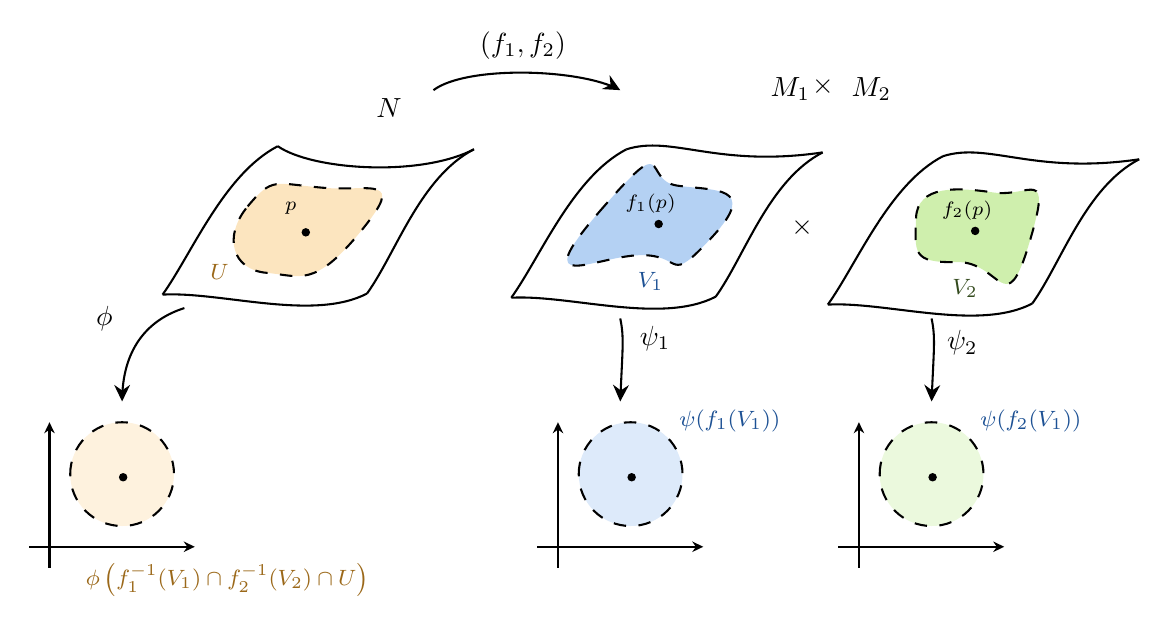
\begin{tikzpicture}[x=0.75pt,y=0.75pt,yscale=-1,xscale=1]
		%uncomment if require: \path (0,300); %set diagram left start at 0, and has height of 300
		
		%Curve Lines [id:da10777202147976128] 
		\draw    (89.5,138.5) .. controls (103.5,119) and (119,80.5) .. (145,67) ;
		%Curve Lines [id:da9226409814736687] 
		\draw    (89.5,138.5) .. controls (118,137) and (162,151.5) .. (188,138) ;
		%Curve Lines [id:da6153501766442295] 
		\draw    (188,138) .. controls (202,118.5) and (213.5,82) .. (239.5,68.5) ;
		%Curve Lines [id:da8299437341096081] 
		\draw    (145,67) .. controls (161.5,78.5) and (213.5,82) .. (239.5,68.5) ;
		%Curve Lines [id:da708998797665932] 
		\draw    (257.5,140) .. controls (271.5,120.5) and (287,82) .. (313,68.5) ;
		%Curve Lines [id:da5763078865113123] 
		\draw    (257.5,140) .. controls (286,138.5) and (330,153) .. (356,139.5) ;
		%Curve Lines [id:da17448723811544053] 
		\draw    (356,139.5) .. controls (370,120) and (381.5,83.5) .. (407.5,70) ;
		%Curve Lines [id:da5843329628503129] 
		\draw    (313,68.5) .. controls (335,61.5) and (356.5,77.5) .. (407.5,70) ;
		%Shape: Polygon Curved [id:ds719249129813768] 
		\draw  [fill={rgb, 255:red, 245; green, 166; blue, 35 }  ,fill opacity=0.29 ][dash pattern={on 4.5pt off 4.5pt}] (130.5,96) .. controls (142.5,81.5) and (143.5,85) .. (166.5,87) .. controls (189.5,89) and (207.5,80.5) .. (185,108) .. controls (162.5,135.5) and (156,129.5) .. (139.5,128) .. controls (123,126.5) and (118.5,110.5) .. (130.5,96) -- cycle ;
		%Shape: Polygon Curved [id:ds20297397591709365] 
		\draw  [fill={rgb, 255:red, 74; green, 144; blue, 226 }  ,fill opacity=0.41 ][dash pattern={on 4.5pt off 4.5pt}] (300,98.5) .. controls (335.5,57.5) and (320,83.5) .. (337.5,86) .. controls (355,88.5) and (377,86) .. (354.5,110.5) .. controls (332,135) and (341,119) .. (319.5,119.5) .. controls (298,120) and (264.5,139.5) .. (300,98.5) -- cycle ;
		%Straight Lines [id:da8177031700071737] 
		\draw    (35,203) -- (35,270) ;
		\draw [shift={(35,200)}, rotate = 90] [fill={rgb, 255:red, 0; green, 0; blue, 0 }  ][line width=0.08]  [draw opacity=0] (5.36,-2.57) -- (0,0) -- (5.36,2.57) -- (3.56,0) -- cycle    ;
		%Straight Lines [id:da5847590524068735] 
		\draw    (102,260) -- (25,260) ;
		\draw [shift={(105,260)}, rotate = 180] [fill={rgb, 255:red, 0; green, 0; blue, 0 }  ][line width=0.08]  [draw opacity=0] (5.36,-2.57) -- (0,0) -- (5.36,2.57) -- (3.56,0) -- cycle    ;
		%Shape: Circle [id:dp5757945587417739] 
		\draw  [fill={rgb, 255:red, 245; green, 166; blue, 35 }  ,fill opacity=0.15 ][dash pattern={on 4.5pt off 4.5pt}] (45,225) .. controls (45,211.19) and (56.19,200) .. (70,200) .. controls (83.81,200) and (95,211.19) .. (95,225) .. controls (95,238.81) and (83.81,250) .. (70,250) .. controls (56.19,250) and (45,238.81) .. (45,225) -- cycle ;
		%Straight Lines [id:da9243110317223102] 
		\draw    (280,203) -- (280,270) ;
		\draw [shift={(280,200)}, rotate = 90] [fill={rgb, 255:red, 0; green, 0; blue, 0 }  ][line width=0.08]  [draw opacity=0] (5.36,-2.57) -- (0,0) -- (5.36,2.57) -- (3.56,0) -- cycle    ;
		%Straight Lines [id:da35917271861832445] 
		\draw    (347,260) -- (270,260) ;
		\draw [shift={(350,260)}, rotate = 180] [fill={rgb, 255:red, 0; green, 0; blue, 0 }  ][line width=0.08]  [draw opacity=0] (5.36,-2.57) -- (0,0) -- (5.36,2.57) -- (3.56,0) -- cycle    ;
		%Shape: Circle [id:dp7567118959752777] 
		\draw  [fill={rgb, 255:red, 74; green, 144; blue, 226 }  ,fill opacity=0.19 ][dash pattern={on 4.5pt off 4.5pt}] (290,225) .. controls (290,211.19) and (301.19,200) .. (315,200) .. controls (328.81,200) and (340,211.19) .. (340,225) .. controls (340,238.81) and (328.81,250) .. (315,250) .. controls (301.19,250) and (290,238.81) .. (290,225) -- cycle ;
		%Curve Lines [id:da8387568355499948] 
		\draw    (220,40) .. controls (235.36,28.48) and (286.66,29.4) .. (307.55,38.78) ;
		\draw [shift={(310,40)}, rotate = 208.93] [fill={rgb, 255:red, 0; green, 0; blue, 0 }  ][line width=0.08]  [draw opacity=0] (8.04,-3.86) -- (0,0) -- (8.04,3.86) -- (5.34,0) -- cycle    ;
		%Curve Lines [id:da5596780294001671] 
		\draw    (310,150) .. controls (311.92,159.12) and (311.08,164.55) .. (310.12,187.09) ;
		\draw [shift={(310,190)}, rotate = 272.29] [fill={rgb, 255:red, 0; green, 0; blue, 0 }  ][line width=0.08]  [draw opacity=0] (8.04,-3.86) -- (0,0) -- (8.04,3.86) -- (5.34,0) -- cycle    ;
		%Curve Lines [id:da33319736118491083] 
		\draw    (100,145) .. controls (83.11,150.31) and (70.88,163.53) .. (70.05,187.36) ;
		\draw [shift={(70,190)}, rotate = 270] [fill={rgb, 255:red, 0; green, 0; blue, 0 }  ][line width=0.08]  [draw opacity=0] (8.04,-3.86) -- (0,0) -- (8.04,3.86) -- (5.34,0) -- cycle    ;
		%Shape: Circle [id:dp912491598557873] 
		\draw  [fill={rgb, 255:red, 0; green, 0; blue, 0 }  ,fill opacity=1 ] (157,108.5) .. controls (157,107.67) and (157.67,107) .. (158.5,107) .. controls (159.33,107) and (160,107.67) .. (160,108.5) .. controls (160,109.33) and (159.33,110) .. (158.5,110) .. controls (157.67,110) and (157,109.33) .. (157,108.5) -- cycle ;
		%Shape: Circle [id:dp5874182665613439] 
		\draw  [fill={rgb, 255:red, 0; green, 0; blue, 0 }  ,fill opacity=1 ] (327,104.5) .. controls (327,103.67) and (327.67,103) .. (328.5,103) .. controls (329.33,103) and (330,103.67) .. (330,104.5) .. controls (330,105.33) and (329.33,106) .. (328.5,106) .. controls (327.67,106) and (327,105.33) .. (327,104.5) -- cycle ;
		%Shape: Circle [id:dp6918787727605586] 
		\draw  [fill={rgb, 255:red, 0; green, 0; blue, 0 }  ,fill opacity=1 ] (69,226.5) .. controls (69,225.67) and (69.67,225) .. (70.5,225) .. controls (71.33,225) and (72,225.67) .. (72,226.5) .. controls (72,227.33) and (71.33,228) .. (70.5,228) .. controls (69.67,228) and (69,227.33) .. (69,226.5) -- cycle ;
		%Shape: Circle [id:dp5802827719353891] 
		\draw  [fill={rgb, 255:red, 0; green, 0; blue, 0 }  ,fill opacity=1 ] (314,226.5) .. controls (314,225.67) and (314.67,225) .. (315.5,225) .. controls (316.33,225) and (317,225.67) .. (317,226.5) .. controls (317,227.33) and (316.33,228) .. (315.5,228) .. controls (314.67,228) and (314,227.33) .. (314,226.5) -- cycle ;
		%Curve Lines [id:da5866172687533027] 
		\draw    (410,143.32) .. controls (424,123.82) and (439.5,85.32) .. (465.5,71.82) ;
		%Curve Lines [id:da33769380232352386] 
		\draw    (410,143.32) .. controls (438.5,141.82) and (482.5,156.32) .. (508.5,142.82) ;
		%Curve Lines [id:da5667601010223242] 
		\draw    (508.5,142.82) .. controls (522.5,123.32) and (534,86.82) .. (560,73.32) ;
		%Curve Lines [id:da7766245611502776] 
		\draw    (465.5,71.82) .. controls (487.5,64.82) and (509,80.82) .. (560,73.32) ;
		%Shape: Polygon Curved [id:ds9848033990053162] 
		\draw  [fill={rgb, 255:red, 126; green, 211; blue, 33 }  ,fill opacity=0.37 ][dash pattern={on 4.5pt off 4.5pt}] (452.5,101.82) .. controls (453,85.5) and (472.5,86.82) .. (490,89.32) .. controls (507.5,91.82) and (518.5,75.5) .. (507,113.82) .. controls (495.5,152.14) and (493.5,122.32) .. (472,122.82) .. controls (450.5,123.32) and (452,118.14) .. (452.5,101.82) -- cycle ;
		%Shape: Circle [id:dp8441479070293367] 
		\draw  [fill={rgb, 255:red, 0; green, 0; blue, 0 }  ,fill opacity=1 ] (479.5,107.82) .. controls (479.5,106.99) and (480.17,106.32) .. (481,106.32) .. controls (481.83,106.32) and (482.5,106.99) .. (482.5,107.82) .. controls (482.5,108.65) and (481.83,109.32) .. (481,109.32) .. controls (480.17,109.32) and (479.5,108.65) .. (479.5,107.82) -- cycle ;
		%Straight Lines [id:da4245600664130684] 
		\draw    (425,203) -- (425,270) ;
		\draw [shift={(425,200)}, rotate = 90] [fill={rgb, 255:red, 0; green, 0; blue, 0 }  ][line width=0.08]  [draw opacity=0] (5.36,-2.57) -- (0,0) -- (5.36,2.57) -- (3.56,0) -- cycle    ;
		%Straight Lines [id:da8383634096867163] 
		\draw    (492,260) -- (415,260) ;
		\draw [shift={(495,260)}, rotate = 180] [fill={rgb, 255:red, 0; green, 0; blue, 0 }  ][line width=0.08]  [draw opacity=0] (5.36,-2.57) -- (0,0) -- (5.36,2.57) -- (3.56,0) -- cycle    ;
		%Shape: Circle [id:dp032856070596776865] 
		\draw  [fill={rgb, 255:red, 184; green, 233; blue, 134 }  ,fill opacity=0.28 ][dash pattern={on 4.5pt off 4.5pt}] (435,225) .. controls (435,211.19) and (446.19,200) .. (460,200) .. controls (473.81,200) and (485,211.19) .. (485,225) .. controls (485,238.81) and (473.81,250) .. (460,250) .. controls (446.19,250) and (435,238.81) .. (435,225) -- cycle ;
		%Shape: Circle [id:dp2655157582176253] 
		\draw  [fill={rgb, 255:red, 0; green, 0; blue, 0 }  ,fill opacity=1 ] (459,226.5) .. controls (459,225.67) and (459.67,225) .. (460.5,225) .. controls (461.33,225) and (462,225.67) .. (462,226.5) .. controls (462,227.33) and (461.33,228) .. (460.5,228) .. controls (459.67,228) and (459,227.33) .. (459,226.5) -- cycle ;
		%Curve Lines [id:da36500972985566005] 
		\draw    (460,150) .. controls (461.92,159.12) and (461.08,164.55) .. (460.12,187.09) ;
		\draw [shift={(460,190)}, rotate = 272.29] [fill={rgb, 255:red, 0; green, 0; blue, 0 }  ][line width=0.08]  [draw opacity=0] (8.04,-3.86) -- (0,0) -- (8.04,3.86) -- (5.34,0) -- cycle    ;
		
		% Text Node
		\draw (191,42.4) node [anchor=north west][inner sep=0.75pt]    {$N$};
		% Text Node
		\draw (381,32.4) node [anchor=north west][inner sep=0.75pt]    {$M_{1}$};
		% Text Node
		\draw (241,10.4) node [anchor=north west][inner sep=0.75pt]    {$( f_{1} ,f_{2})$};
		% Text Node
		\draw (318,152.4) node [anchor=north west][inner sep=0.75pt]    {$\psi _{1}$};
		% Text Node
		\draw (56,142.4) node [anchor=north west][inner sep=0.75pt]    {$\phi $};
		% Text Node
		\draw (147,92.4) node [anchor=north west][inner sep=0.75pt]  [font=\scriptsize]  {$p$};
		% Text Node
		\draw (311,88.4) node [anchor=north west][inner sep=0.75pt]  [font=\scriptsize]  {$f_{1}( p)$};
		% Text Node
		\draw (111,122.4) node [anchor=north west][inner sep=0.75pt]  [font=\footnotesize,color={rgb, 255:red, 155; green, 104; blue, 25 }  ,opacity=1 ]  {$U$};
		% Text Node
		\draw (317,126.4) node [anchor=north west][inner sep=0.75pt]  [font=\footnotesize,color={rgb, 255:red, 29; green, 81; blue, 148 }  ,opacity=1 ]  {$V_{1}$};
		% Text Node
		\draw (337,192.4) node [anchor=north west][inner sep=0.75pt]  [font=\footnotesize,color={rgb, 255:red, 29; green, 81; blue, 148 }  ,opacity=1 ]  {$\psi ( f_{1}( V_{1}))$};
		% Text Node
		\draw (51,266.4) node [anchor=north west][inner sep=0.75pt]  [font=\footnotesize,color={rgb, 255:red, 155; green, 104; blue, 25 }  ,opacity=1 ]  {$\phi \left( f_{1}^{-1}( V_{1}) \cap f_{2}^{-1}( V_{2}) \cap U\right)$};
		% Text Node
		\draw (463.5,91.72) node [anchor=north west][inner sep=0.75pt]  [font=\scriptsize]  {$f_{2}( p)$};
		% Text Node
		\draw (468.5,129.72) node [anchor=north west][inner sep=0.75pt]  [font=\footnotesize,color={rgb, 255:red, 52; green, 75; blue, 30 }  ,opacity=1 ]  {$V_{2}$};
		% Text Node
		\draw (482,192.4) node [anchor=north west][inner sep=0.75pt]  [font=\footnotesize,color={rgb, 255:red, 29; green, 81; blue, 148 }  ,opacity=1 ]  {$\psi ( f_{2}( V_{1}))$};
		% Text Node
		\draw (420,32.4) node [anchor=north west][inner sep=0.75pt]    {$M_{2}$};
		% Text Node
		\draw (391,100.4) node [anchor=north west][inner sep=0.75pt]    {$\times $};
		% Text Node
		\draw (466,154.4) node [anchor=north west][inner sep=0.75pt]    {$\psi _{2}$};
		% Text Node
		\draw (401,32.4) node [anchor=north west][inner sep=0.75pt]    {$\times $};
		
		
	\end{tikzpicture}
\end{figure}
	\FloatBarrier
	
	For the first direction, we will show that smoothness of $ (f_1,f_2): N \to M_1\times M_2 $ implies the smoothness of $ f_1:N\to M_1 $ and $ f_2: N \to M_2 $. As depicted in the picture above, let $ \phi $ be a coordinate map for $ N $ and $ \psi_1, \psi_2 $ be coordinate maps for $ M_1,M_2 $ respectively. Since $ (f_1,f_2) $ is smooth, then $ (\psi_1 \times \psi_2) \circ (f_1,f_2) $ is smooth. Let $ p \in N $, then
	\[ ((\psi_1 \times \psi_2) \circ (f_1,f_2) \circ \inv{\phi})(\phi(p)) =
	((\psi_1 \times \psi_2) \circ (f_1,f_2)) (p) = (\psi_1\times \psi_2)(f_1(p),f_2(p)) = (\psi_1(f_1(p)), \psi_2(f_2(p))).
	 \]
	This is a smooth map from $ \R^n $ to $ \R^{m_1+m_2} $. Thus the components of the function are also smooth.
	
	For the converse, we need to show that the smoothness of $ f_1 $ and $ f_2 $ implies the smoothness of $ (f_1,f_2) $. Similar to the argument above, the smoothness of $ (f_1,f_2) $ follows immediately from the smoothness of the components.
\end{solution}

\begin{problem}[Smooth functions on unit circle (W. Tu)]
	We have studied before that the unit circle $ S^1 $ defined by $ x^2 + y^2 = 1 $ in $ \R^2 $ is a $ C^\infty $ manifold. Prove that a smooth function $ f: \R^2 \to \R $ defined on $ \R^2 $ restricts to a $ C^\infty $ function on $ S^1 $.
\end{problem}

\begin{solution}
	Consider the following inclusion map
	\[ i: S^1 \to \R^2 \]
	defined as $ i(p) = (x(p),y(p)) $, where $ x,y $ are the standard coordinate functions. The restriction of $ f $ to manifold will be
	\[ f|_{S^1} = f \circ i. \]
	To show that $ f|_{S^1} $ is smooth, we just need to show that the inclusion map is smooth. To show this we need to show that the components of this vector valued function is smooth. We start by showing that $ x $ is smooth. We use the same charts as in \autoref{problem:S^1Charts}. Let $ p \in S^1 $. If $ p \in U_3 \cap U_4 $ then we have
	\[ \mathds{1}_{(0,1)}\circ x \circ \inv{\phi_3} = \mathds{1}_{(0,1)}: (-1,1) \to \R^2, \qquad \mathds{1}_{(0,1)}\circ x \circ \inv{\phi_4} = \mathds{1}_{(0,1)}: (-1,1) \to \R^2,  \]
	which are both identity maps, thus smooth. So $  x $ is smooth on $ U_3\cap U_4 $. For $ U_1 $ we have
	\[ \mathds{1}_{(0,1)}\circ x \circ \inv{\phi_1}(x) = -\sqrt{1-x^2}, \qquad\text{for } x \in \phi_1(U_1) = (-1,1) \]
	thus $ x $ is smooth on $ U_1 $ as well. For $ U_2 $ we have
	\[ \mathds{1}_{(0,1)}\circ x \circ \inv{\phi_2}(x) = \sqrt{1-x^2}, \qquad\text{for } x \in \phi_2(U_2) = (-1,1) \]
	thus $  x $ is smooth on $ U_2  $ as well. We can use a similar strategy to show that the coordinate function $ y $ is also smooth.
\end{solution}



\begin{problem}
	The general linear group $ \operatorname{GL}(n,\R) $ is the set of all real valued matrices with non-zero determinant under matrix multiplication. In other words
	\[ \operatorname{GL}(n,\R) = \set{A = \left[ a_{ij} \right] \in \R^{n\times n}\ |\ \det(A) \neq 0} . \]
	We can see this as an open subset of $ \R^{n\times n} $, thus it is a manifold. Show that this forms a Lie group.
\end{problem}

\begin{solution}
	Let $ A,B $ be two matrices in the manifold. Then the $ i,j $ element of $ AB $ is
	\[ (AB)_{ij} = \sum_{k=1}^{n} A_{ik}B_{kj} \]
	which is a polynomial in the coordinates of $ A $ and $ B $, thus it is smooth. To show that the inverse is also smooth, for any function $ A $ in the manifold we have
	\[ \inv{A} = \frac{1}{\det(A)} \cdot (-1)^{i+j}((i,j)\text{- minor of $ A $}). \]
	The $ (i,j)\text{-minor} $ of matrix $ A $ is the determinant of the sub matrix by deleting the $ i\text{-th} $ row and $ j\text{th} $ column, which is again a polynomial in the coordinates of $ A $ and $ B $, thus smooth (given that $ \det(A) \neq 0 $).
\end{solution}

\begin{problem}[Jacobian matrix os a transition map (form W. Tu)]
	Let $ (U,\phi) = (U,x^1,\cdots,x^n) $ and $ (V,\psi) = (V,y^1,\cdots,y^n) $ be overlapping charts on a manifold $ M $. The transition map $ \psi \circ\inv{\phi}: \phi(U\cap V) \to \psi(U\cap V) $ is a diffeomorphism of open subsets of $ \R^n $. Show that its Jacobian matrix $ J(\psi\circ\inv{\phi}) $ at $ \phi(p) $ is the matrix $ [\partial y^i/\partial x^j] $ of partial derivatives at $ p $.
\end{problem}
\begin{solution}
	From the definition of the Jacobian matrix we can write
	\[ J(\psi \circ \inv{\phi}) = \frac{\partial (\psi \circ \inv{\phi})^i}{\partial r^j} =  \frac{\partial (r^i \circ \psi \circ \inv{\phi})}{\partial r^j} = \frac{\partial (y^i \circ \inv{\phi})}{\partial r^j} = \frac{\partial y^i}{\partial x^j}. \]
\end{solution}

\begin{observation}[Some mnemonics for the Jacobian matrix]
	Here I introduce a symbolic mnemonic of remembering the form of the Jacobian matrix of a smooth map between manifolds. Let $ F:N\to M $ a smooth map between manifolds. Since this function is from $ N $ to $ M $, then the Jacobian matrix will be of the form
	\[ J(F) = [\partial F^i / \partial x^j] \] 
	where $ x^j $ a local coordinate in $ N $ and $ F^i = y^i \circ F $ where $ y^i $ is a local coordinate in $ M $. What we mean by local coordinates here is that for a point $ p $ on the manifold for which we want to calculate the Jacobian matrix, there are charts $ (U,x^1\cdots,x^n) $ and $ (V,y^1,\cdots,y^n) $ on $ N $ and $ M $ respectively such that $ p \in U $ and $ F(U) \subset V $.
	
	As another example, in the question above, since the function $ \psi\circ\inv{\phi} $ is defined from $ \R^n \to \R^n $, then the Jacobian of this function starts with coordinates of $ \R^n $, i.e. $ r^i $.
\end{observation}

\begin{problem}[From W. Tu]
	Find all points in $ \R^2 $ in a neighborhood of which the functions given by $ x^2 + y^2 -1  $ and $ y $ can serve as a local coordinate system.
\end{problem}
\begin{solution}
	Define $ F^1(x,y) = x^2 + y^2 -1 $ and $ F^2(x,y) = y  $. Then the pair $ (F^1,F^2) $ is locally invertible, thus can serve as a local diffeomorphism to $ \R^2 $, thus a coordinate map if the Jacobian determinant $ [\partial F^i /\partial x^i] $ is not zero. I.e.
	\[ \det\matt{2x}{2y}{0}{1} = 2x \neq 0 \implies x \neq 0. \]
	Thus the function $ F = (F^1,F^2) $ can act as a local coordinate map everywhere except for on the points on the $ y $ axis. You can see why this happens in the plots below. As you can see, any path that is not crossing the $ y $ axis with zero vertical velocity is diffeormorphically mapped to an smooth curve. But when the curve passes through the $ y $ axis with a zero vertical velocity, then the curve folds on itself when mapped by $ F $, thus $ F $ fails be locally invertible and thus fails to be a coordinate map. Thus for any point that is not on the $ y $ axis, we can find an open set small enough that does not overlap with the $ y $ axis. But there is no such an open ball for the points on the $ y $ axis.	You can try the online plotting tool that I have configured to generate the following plots \href{https://www.desmos.com/calculator/pam0whmnbs}{here}.
	\begin{figure}[h!]
		\centering
		\includegraphics[width=0.8\linewidth]{Images/diffeomorphismExample}
	\end{figure}
	
\end{solution}

\begin{problem}[Differentiable structure on $ \R $]
	Let $ \R $ be the real line with the differentiable structure given by the maximal atlas of the chart $ (\R, \phi=\mathds{1}:\R \to \R) $, and let $ \R' $ be the real line with the differentiable structure given by the maxima atlas of the chart $ (\R, \psi:\R\to\R) $, where $ \psi(x) = x^{1/3} $.
	\begin{enumerate}[(a)]
		\item Show that these two differentiable structures are distinct.
		\item Show that there is a diffeomorphism between $ \R $ and $ \R' $. (\emph{Hint:} The identity map $ \R \to \R  $ is not  the desired diffeomorphism; in fact, this map is not smooth).
	\end{enumerate}
\end{problem}
\begin{solution}
	\begin{enumerate}[(a)]
		\item Let $ M_1 $ be the atlas containing $ (\R,\phi) $ and $ M_2 $ the atlas containing $ (\R,\psi) $. Assume $ M_1 = M_2 $. Then $ (\R,\phi) $ should be compatible with $ (\R,\psi) $, i.e. the functions
		\[ \psi \circ \inv{\phi} = \R \to \R, \qquad \phi\circ \inv{\psi}:\R \to \R, \]
		are smooth. This is not true since $ (\psi \circ \inv{\phi} )(x) = x^{1/3} $ that is not differentiable at $ x=0 $. So $ M_1 \neq M_2 $ and these two atlases are distinct.
		\item For a more clear demonstration, the manifold with atlas generated by $ (\R,\phi=\mathds{1}:\R\to \R) $ the manifold $ R $, and call the other manifold the manifold $ R' $. Define the map $ F $ between manifolds
		\[ F: R \to R' \]
		as $ F(p) = p^3 $ for $ p \in R $. The inverse of this map will be $ \inv{F}(p) = p^{1/3} $. To show this map is a diffeomorphism, we need to show that the following 
		\[ \psi \circ F \circ \inv{\phi}: \phi(U)\to \psi(F(U)), \qquad \phi\circ\inv{F}\circ\inv{\phi}: \phi(V) \to \phi(\inv{F}(V)), \]
		are smooth. In  equations above, $ (U,\phi: x\mapsto x) $ is some coordinate system (i.e. chart) on $ R $ whereas $ (V,\psi: x\mapsto x^1/3) $ is a coordinate system on $ R' $. Let $ \phi(x) = x \in \phi(U\cap V) $. Then
		\[ (\psi\circ F \circ\inv{\phi})(x) = \psi(F(x)) = \psi(x^3) = x,\]
		which is the identity map and is smooth. Furthermore
		\[( \phi\circ\inv{F}\circ\inv{\phi})(x) = \phi(F^{-1}(x^3)) = \psi(x) = x,\]
		which is again the identity map and is smooth. Thus the map $ F $ is a diffeomorphism between the manifolds.
	\end{enumerate}
\end{solution}


\begin{problem}[The smoothness of an inclusion map (From L. Tu)]
	Let $ M $ and $ N $ be manifolds and let $ q_0 $ be a point in $ N $. Prove that the inclusion map $ i_{q_0}: M \to M\times N $, $ i_{q_0}(p) = (p,q_0) $, is $ C^\infty $.
\end{problem}
